\section{Deep Learning}

\subsection{Revision of Deep Learning}
Deep learning is a rapidly developing field within machine learning that has recently got significant attention within economics.
The idea is to transform complex data into a series of simpler representations, each of which is expressed in terms of the previous one \citep{Goodfellow-et-al-2016}.
A common example of this is the \textit{feedforward neural network} architecture, which consists of a series of layers of neurons, each of which is connected to the next layer.
The first layer is the input layer, the last layer is the output layer, and the layers in between are called hidden layers.
The input layer corresponds to the covariates $X$, the output layer corresponds to the outcome $Y$.
Figure \ref{fig:1} illustrates the layer and node structure of a \ac{mlp}, which is a special class of feed forward networks and is commonly used in empirical applications \citep{farrellDeepNeuralNetworks2021}.
In this thesis, I use \ac{mlp} and deep learning interchangeably as it is the approach used here.

The actual computation within the neural networks is done by the \textit{activation function} $ \sigma : \mathbb{R} \to \mathbb{R} $, which is applied to the output of each hidden neuron.
The most common activation function is the \ac{relu} function, defined as $ \sigma(x) = \max(0, x) $, which is used in this thesis.
The advantage of the linear \ac{relu} is its computational efficiency and its ability to circumvent the vanishing gradient problem, which is a common problem in deep learning \citep{10.1214/19-AOS1875}.
\footnote[1]{The vanishing gradient issue arises especially by activation functions like \textit{sigmoid} and \textit{tanh}.
When the neural network model is trained, all the weights of the model are updated through a process called \textit{backpropagation}.
Backpropagation is the algorithm used to compute the gradient of the loss function with respect to each parameter, which is then used to update the parameters such that they minimizes the loss.
The issue that can arise is that updating of parameters is hindered or training is completely stopped \citep{abuqaddom2021oriented}.}
The \ac{relu} takes any linear combination given by $\tilde{x}' w + b$ and transforms it to $ \sigma(\tilde{x}' w + b)$, where $w$ is the weight vector, $b$ is the constant term\footnote[2]{The actual term in computer science is \textit{bias} but to avoid confusion with econometric term I, follow \citet{farrellDeepNeuralNetworks2021} and use the term \textit{constant}}
, and $\tilde{x}$ is the input vector.
Thus, the \ac{relu} function sets all negative values from the linear combination $\tilde{x}' w + b$ to zero, while keeping all positive values unchanged.

\begin{figure}%                 use [hb] only if necceccary!
\centering
\caption{Illustration of a feedforward neural network \citep{farrellDeepNeuralNetworks2021}}
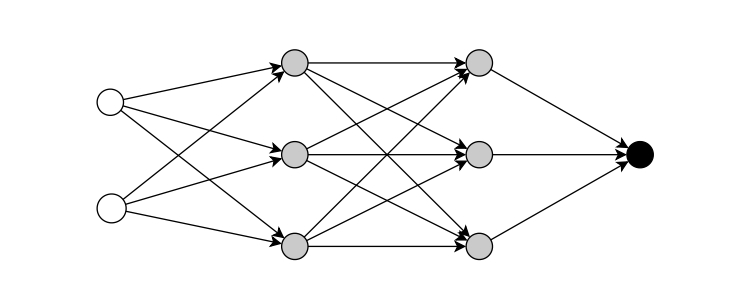
\includegraphics[width=\textwidth]{Neural_net}
\caption*{Note: This figure illustrates the basic structure of a \ac{mlp} $\mathcal{F}_{\text{MLP}}$, showing the input layer with $d=2$ neurons in white. The two ($H=2$) hidden layers in grey with $U=6$ neurons, and one output layer in black ($L=1$). The total amount of weights is $W=28$.}
\label{fig:1}
\end{figure}


The main problem the neural network aims to solve is estimating the unknown function $f^*(x)$.
More precisely, $f^*$ is a function that maps the input $\tilde{x}$ to the output $\tilde{y}$.
As $f^*$ is unknown, the neural network tries to estimate it by minimizing the expected loss function $\mathbb{E}[\ell(f, Z)]$, which can be written as:
\begin{equation}
f^* = \arg \min_f \mathbb{E}[\ell(f, Z)],
\end{equation}
where $\ell(f, Z)$ is the loss function, and the function $f$ predicts the outcome $\hat{Y} = f(X)$ and $Z = (Y, X')' \in \mathbb{R}^{d+1}$ is the set of random variables.
The loss function can take various forms, such as least squares or logistic regression, with the latter used for propensity score estimation in this paper.
The logistic loss function is therefore defined as follows:
\begin{equation}
f^*(x) := \log \left( \frac{\mathbb{E}[Y|X = x]}{1 - \mathbb{E}[Y|X = x]} \right) \quad \text{and} \quad \ell(f, z) = -yf(x) + \log(1 + e^{f(x)}).
\label{eq:8}
\end{equation}
The logistic regression in eq. \ref*{eq:8} is a method used for binary classification and estimates the probability that the covariates $X$ take on values $0$ or $1$.
The loss function measures the difference between the estimated probabilities and the actual class values.
Unlike simple logistic regression applications, deep learning minimizes the loss function $\ell(f, z)$ by updating iteratively the weights and constants.
For this $Z$ is passed multiple times through the neural network until the loss is minimized.
The amount of iterations is called \textit{epochs}.

Combining all the elements described above, the full neural network can be formalized trough recursion:
\begin{equation}
\hat{f}_{\text{MLP}}(x) = W_L \sigma \left( \cdots \sigma \left( W_3 \sigma \left( W_2 \sigma \left( W_1 \sigma \left( W_0 x + b_0 \right) + b_1 \right) + b_2 \right) + b_3 \right) + \cdots \right) + b_L,
\label{eq:9}
\end{equation}
where $\hat{f}$ can be interpreted as a series of nested functions, where each function is a linear combination of the previous function.
Note that $W_l$ is the weight matrix for layer $l$.
Equation \ref{eq:9} shows how the \ac{relu} activation function $sigma$ is applied to each hidden layer, starting with the covariates $x$.
The transformed output of each hidden layer becomes the input for the next layer, and this process continues iteratively until the loss function is minimized.
During this iterative process, the weights $W$ and biases $b$ are adjusted using the gradients computed from the loss function, typically through gradient descent.
This ensures that the network parameters are optimized to improve prediction accuracy.

Equation \ref{eq:10} shows an example of a neural network with $L$ hidden layers and the final output layer:
\begin{align}
h_1 &= \sigma(W_1 X + b_1), \nonumber \\
h_2 &= \sigma(W_2 h_1 + b_2), \nonumber  \\
&\vdots \nonumber \\
h_L &= \sigma(W_L h_{L-1} + b_L),
\label{eq:10}
\end{align}
Finally, the output of the network is:
\begin{equation}
\hat{Y} = W_L h_{L-1} + b_L, \nonumber
\end{equation}



Some final remarks to the neural networks in general.
First, if deep learning practitioners mention tuning parameters than they refer to the width and depth of the network, e.g. the amount of hidden layers \citep{farrellDeepNeuralNetworks2021}.
These parameters are also the ones on which the neural network is repeatedly trained.
Secondly, unlike inference, there is no understanding within the deep learning literature how to select the optimal architecture or tuning parameters \citep[see][]{10.1214/19-AOS1875,telgarsky2016benefits}.
Consequently, the chosen neural network architecture may not be the optimal one, and selecting the right architecture is often arbitrary.
\subsection{Deep Learning for Inference}
%first cite farrel paper where they describe the two use cases of semiparametric ML stuff
The recent applications of deep learning for inferences mostly focusses on prediction problems, such as outcome or propensity score prediction.
The idea is to embed the neural network within a semiparametric framework, where the neural network is used to estimate the unknown function $f^*$.
In this framework, neural network is used as a first-step estimator, where the fitted values of the neural network are used as the input for the second-step inference. %is this correct?
Other techniques such as tree-based methods, logistic regression, or hybrid models are also used as first-step estimators.
The advantage of these machine learning approaches is that they considered to perform well under heterogenous treatment effects, conditional controls or many covariates \citep{belloni2017program}.
\citet{belloni2017program} show that neural network perform as well as other machine learning approaches in terms of recovering the true treatment effect as a first step estimator.
\citet{chernozhukovDoubleDebiasedMachine2018} approves those results even in a low-dimensional setting but struggle with the neural net if $n$ is small.
Common across literature are the benefits of deep learning regarding handling heterogenous treatment effects \citep[see][]{DeepLearningIndividual2021,belloni2017program,chernozhukovDoubleDebiasedMachine2018}

Another major advantage of Deep learning is its effectiveness in a high covariate settings \citep{chernozhukov2022automatic}\footnote[3]{\citet{belloni2017program} demonstrates this for \textit{moderately high} and \textit{very high} covariates compared to the sample size.}.
This advantage arises from deep learning's capability to perform variable selection.
Especially employing some form of regularization makes deep learning a useful tool \citep{chernozhukovDoubleDebiasedMachine2018} particular by reducing the variance induced by high covariates but comes at the costs of higher bias.
Many machine learning techniques (see lasso or some tree-based methods) have similar properties.
As such this thesis does not try to promote deep learning as an optimal technique but aims to investigate its utility as a valid first-step estimator in a semiparametric \ac{did} framework.

To evaluate deep learnings performance, there are multiple important criterias to consider.
First, deep learning should have good approximation power \citep{belloni2017program}, meaning it can closely approximate the true underlying function of the data.
Second, deep learning should avoid overfitting of the data \citep{belloni2017program}, leading to poor generalization on new data.
%explain what that means and how one can see that
Third, \citet{belloni2017program} emphasize that doubly robust estimation methods ensure valid inference for many machine learning frameworks. including neural networks.\footnote[4]{\citet{belloni2017program} also point out that some form of orthogonal moment condition can also lead to valid inference in this setting. See \citet{DeepLearningIndividual2021} for a discussion that with even weaker conditions than doubly robust or orthogonality valid semiparametric inference is achievable, although these are not of focus here.}.

% why to use deep learning for inference
% farrell, chernozhukov et al, belloni et al


%how to use deep learning for inference
%see what farrell wrote to OR and propensity score estimation with deep learning

%how my paper uses deep learning
